\documentclass[11pt,a4paper]{article}
\usepackage[margin=2.2cm]{geometry}
\usepackage{amsmath,amssymb}
\usepackage{graphicx}
\usepackage{booktabs,array,tabularx,multirow}
\usepackage{xcolor}
\usepackage{xurl}
\usepackage[hidelinks]{hyperref}
\usepackage{enumitem}
\usepackage{caption}
\usepackage{float}
\captionsetup{font=small,labelfont=bf}
\setlist{itemsep=2pt,topsep=4pt}
\newcolumntype{L}{>{\raggedright\arraybackslash}X}
\newcommand{\code}[1]{\texttt{\small #1}}
\definecolor{plan}{rgb}{0.75,0.1,0.1}
\newcommand{\todo}[1]{{\color{plan}\textbf{[TODO:} #1\textbf{]}}}
\newcommand{\demo}{{\color{plan}\textsc{placeholder}}}
\newcommand{\ph}[2]{\fbox{\parbox[c][#1][c]{0.95\linewidth}{\centering\color{gray}\small #2}}}
\newcommand{\nue}{\ensuremath{\nu_e}}
\newcommand{\numu}{\ensuremath{\nu_\mu}}

\title{\textbf{Learning Charge--Light Correlations:\\ A Multi-Modal Foundation Model for Liquid-Argon TPCs}\\[4pt]
\large Paper plan and initial draft (v0)}
\author{Haiwang Yu et al.\thanks{Prepared with the assistance of Claude (Anthropic). Code: \url{https://github.com/HaiwangYu/fm4npp-lartpc}. Tracking: \code{docs/paper-campaign.md} and GitHub issue \#7. Every figure and number marked \demo{} comes from tech notes 1--4 (\code{docs/technote-round\{1..4\}.pdf}) and will be replaced by the campaign runs.}}
\date{Draft v0, November 2026}

\begin{document}
\maketitle

\begin{center}\fbox{\parbox{0.93\linewidth}{\small
\textbf{How to read this draft.} Black text is meant to survive into the paper (in rough form). {\color{plan}Red} marks plan items, TODOs and placeholders. Figures and tables are \demo{}s from the tech notes, each with a note on how the final version differs. Appendix~\ref{app:plan} is the campaign plan: decisions, the Section-2 job plan ($\leq$200 node-hours), timeline and venue.}}\end{center}

\begin{abstract}
\noindent
Foundation models (FMs) pretrained with self-supervision are changing how detector data are analysed, but the FMs proposed for liquid-argon time projection chambers (LArTPCs) see only the ionization charge. LArTPCs also record scintillation light, which gives the event time and an independent calorimetric view. We present a multi-modal FM that reads low-level charge hits from three wire planes and the waveforms of 32 photomultipliers as one token sequence, and is pretrained without labels on MicroBooNE open data. On five tasks -- $\nu$ hit identification, $\nu$/cosmic event classification, flavour, energy and charge$\to$light prediction -- light helps every model, but learning the charge--light correlation \emph{during pretraining} (early fusion) is what matters: the same backbone pretrained on charge alone, with light added afterwards by a strong cross-attention head, recovers only part of the gain. The correlation is learned from 2D wire-plane data, without an explicit 3D reconstruction. We compare four FM recipes -- a Transformer with masked autoencoding, a Transformer with a joint-embedding predictive objective, a Point Transformer V3 with self-distillation, and a Mamba-2 state-space model -- with light in pretraining at matched size and compute. \todo{one sentence with the Section-2 outcome.}
\end{abstract}

\tableofcontents
\newpage

%=====================================================================
\section{Introduction}\label{sec:intro}
{\color{plan}\textit{Outline (about 1 page). References from \code{docs/survey-round1.pdf}.}}
\begin{enumerate}
  \item \textbf{FMs work for detector data.} Self-supervised pretraining on unlabelled detector data gives reusable representations that reduce label needs and transfer across tasks: masked particle modelling on jets~\cite{mpm,mpmv2}, PoLAr-MAE~\cite{polarmae} and Panda~\cite{panda,pandav2} on LArTPC charge, FM4NPP on a TPC~\cite{fm4npp}, heterogeneous neutrino detectors~\cite{fasercal}; review in~\cite{hallin}.
  \item \textbf{Multi-modal FMs are better where modalities are complementary.} Masked multi-modal modelling (MultiMAE~\cite{multimae}) and science omnimodal models (AION-1~\cite{aion}) learn cross-modal structure; in HEP, tokenized any-to-any models map between levels of the reconstruction chain~\cite{prompting,heptokens}. Native early-fusion models do at least as well as late fusion and are better at small sizes~\cite{shukor}.
  \item \textbf{The gap: LArTPC FMs are charge-only.} The scintillation light carries the event time $t_0$ (which fixes the drift coordinate) and an independent energy measure; conventional reconstruction uses it only after 3D reconstruction, through flash matching~\cite{pandora}. To our knowledge no LArTPC FM pretrains on charge and light together.
  \item \textbf{Contributions.}
  \begin{itemize}
    \item The first multi-modal (charge + light) self-supervised FM for LArTPCs, on low-level data (hits after signal processing, optical hits) with no high-level reconstruction.
    \item A controlled study showing that the gain comes from correlations learned in pretraining, not from having light at the input (early vs late fusion; shortcut-controlled metrics).
    \item A compute-matched comparison of four FM recipes with light in pretraining (Section~\ref{sec:arch}).
    \item Analysis of how the correlation is learned: probes, fusion depth, an oracle 3D input (Section~\ref{sec:how}).
    \item A five-task benchmark on MicroBooNE open data with Pandora references. \todo{decide whether to release splits/code as a benchmark.}
  \end{itemize}
\end{enumerate}

%=====================================================================
\section{Data, tasks and models}\label{sec:setup}
\paragraph{Data.} MicroBooNE BNB inclusive and \nue{} CC overlay samples (NoWire HDF5 open data, Zenodo 8370883 and 7261921): simulated neutrinos on real off-beam cosmic data, about 831k events. Inputs: reconstructed wire hits of the three planes (after signal processing and hit finding) and optical hits of the 32 PMTs in a 24\,$\mu$s window. No Pandora output is used as model input. Splits: 90\% pretraining pool, labelled pools of 0.1\%, 1\%, 10\%, 100\%; fixed validation and test subsets (TN1).

\paragraph{Tasks and metrics} {\color{plan}(updated from the tech notes to avoid trivial learning)}.
\begin{table}[H]\centering\footnotesize
\caption{Downstream tasks. {\color{plan}Changes from the tech notes in red.}}\label{tab:tasks}
\begin{tabularx}{\textwidth}{lLL}\toprule
Task & Target & Headline metric\\\midrule
T1 & per-hit $\nu$ vs cosmic & {\color{plan}per-event F1 of $\nu$ hits, unweighted median over events} (up-weights small, hard events; TN4 used charge-weighted)\\
T2 & event: in-AV $\nu$ / out-of-AV $\nu$ / no $\nu$ & {\color{plan}AUC in-AV vs no-$\nu$ on events passing the 200\,PE beam-flash cut} (TN4), where flash presence alone gives only AUC 0.69\\
T3 & flavour: \numu{} CC / \nue{} CC / NC & macro-F1 (as TN1)\\
T4 & $\log E_\nu$ for CC, fiducial & {\color{plan}resolution on a truth-based clean subset, the same for every model}: CC, fiducial vertex, $\nu$ carries $\geq$5\% of the event charge (keeps 69\%; median 7\%), visible fraction $E_{\rm dep}/E_\nu\geq0.3$ (containment proxy); all eligible events in the appendix\\
T5 & charge $\to$ 32 PMT $\times$ 17 light features & test MSE in $\log(1+\mathrm{PE})$; total-PE resolution on $\geq$200\,PE events\\
\bottomrule\end{tabularx}
\end{table}

\paragraph{Models.} Each model = tokenizer + backbone + SSL objective + downstream heads, about 20M parameters.
\begin{itemize}
  \item \textbf{qlfm-M CL} (main): charge cells (16 wires $\times$ 64 ticks) and 32 PMT tokens in one sequence; 12-layer Transformer, $d=384$; masked autoencoding (MAE~\cite{mae}) over both modalities. \textbf{qlfm-M C}: identical, pretrained on charge only.
  \item \textbf{PTv3 + Sonata}: Point Transformer V3~\cite{ptv3} with Sonata self-distillation~\cite{sonata}, the recipe of Panda~\cite{panda}, size-matched (21M). {\color{plan}In the paper: ``PTv3 (as used in Panda)''; we do not use Panda's weights.}
  \item \textbf{Pandora}~\cite{pandora}: the reconstruction in the open data, used directly ($\nu$ slice, $\nu$ score) and through a BDT on 32 Pandora features (+ 8 light features).
  \item Section~\ref{sec:arch} adds Transformer + JEPA~\cite{ijepa} and Mamba-2~\cite{mamba2} (FM4NPP recipe~\cite{fm4npp}), each with light.
\end{itemize}
\paragraph{Heads.} Frozen backbone + head; single-task fine-tune (TN1--4); {\color{plan}new: multi-task fine-tune, one backbone and five heads trained together}, which is how an FM would be deployed.

\begin{figure}[H]\centering
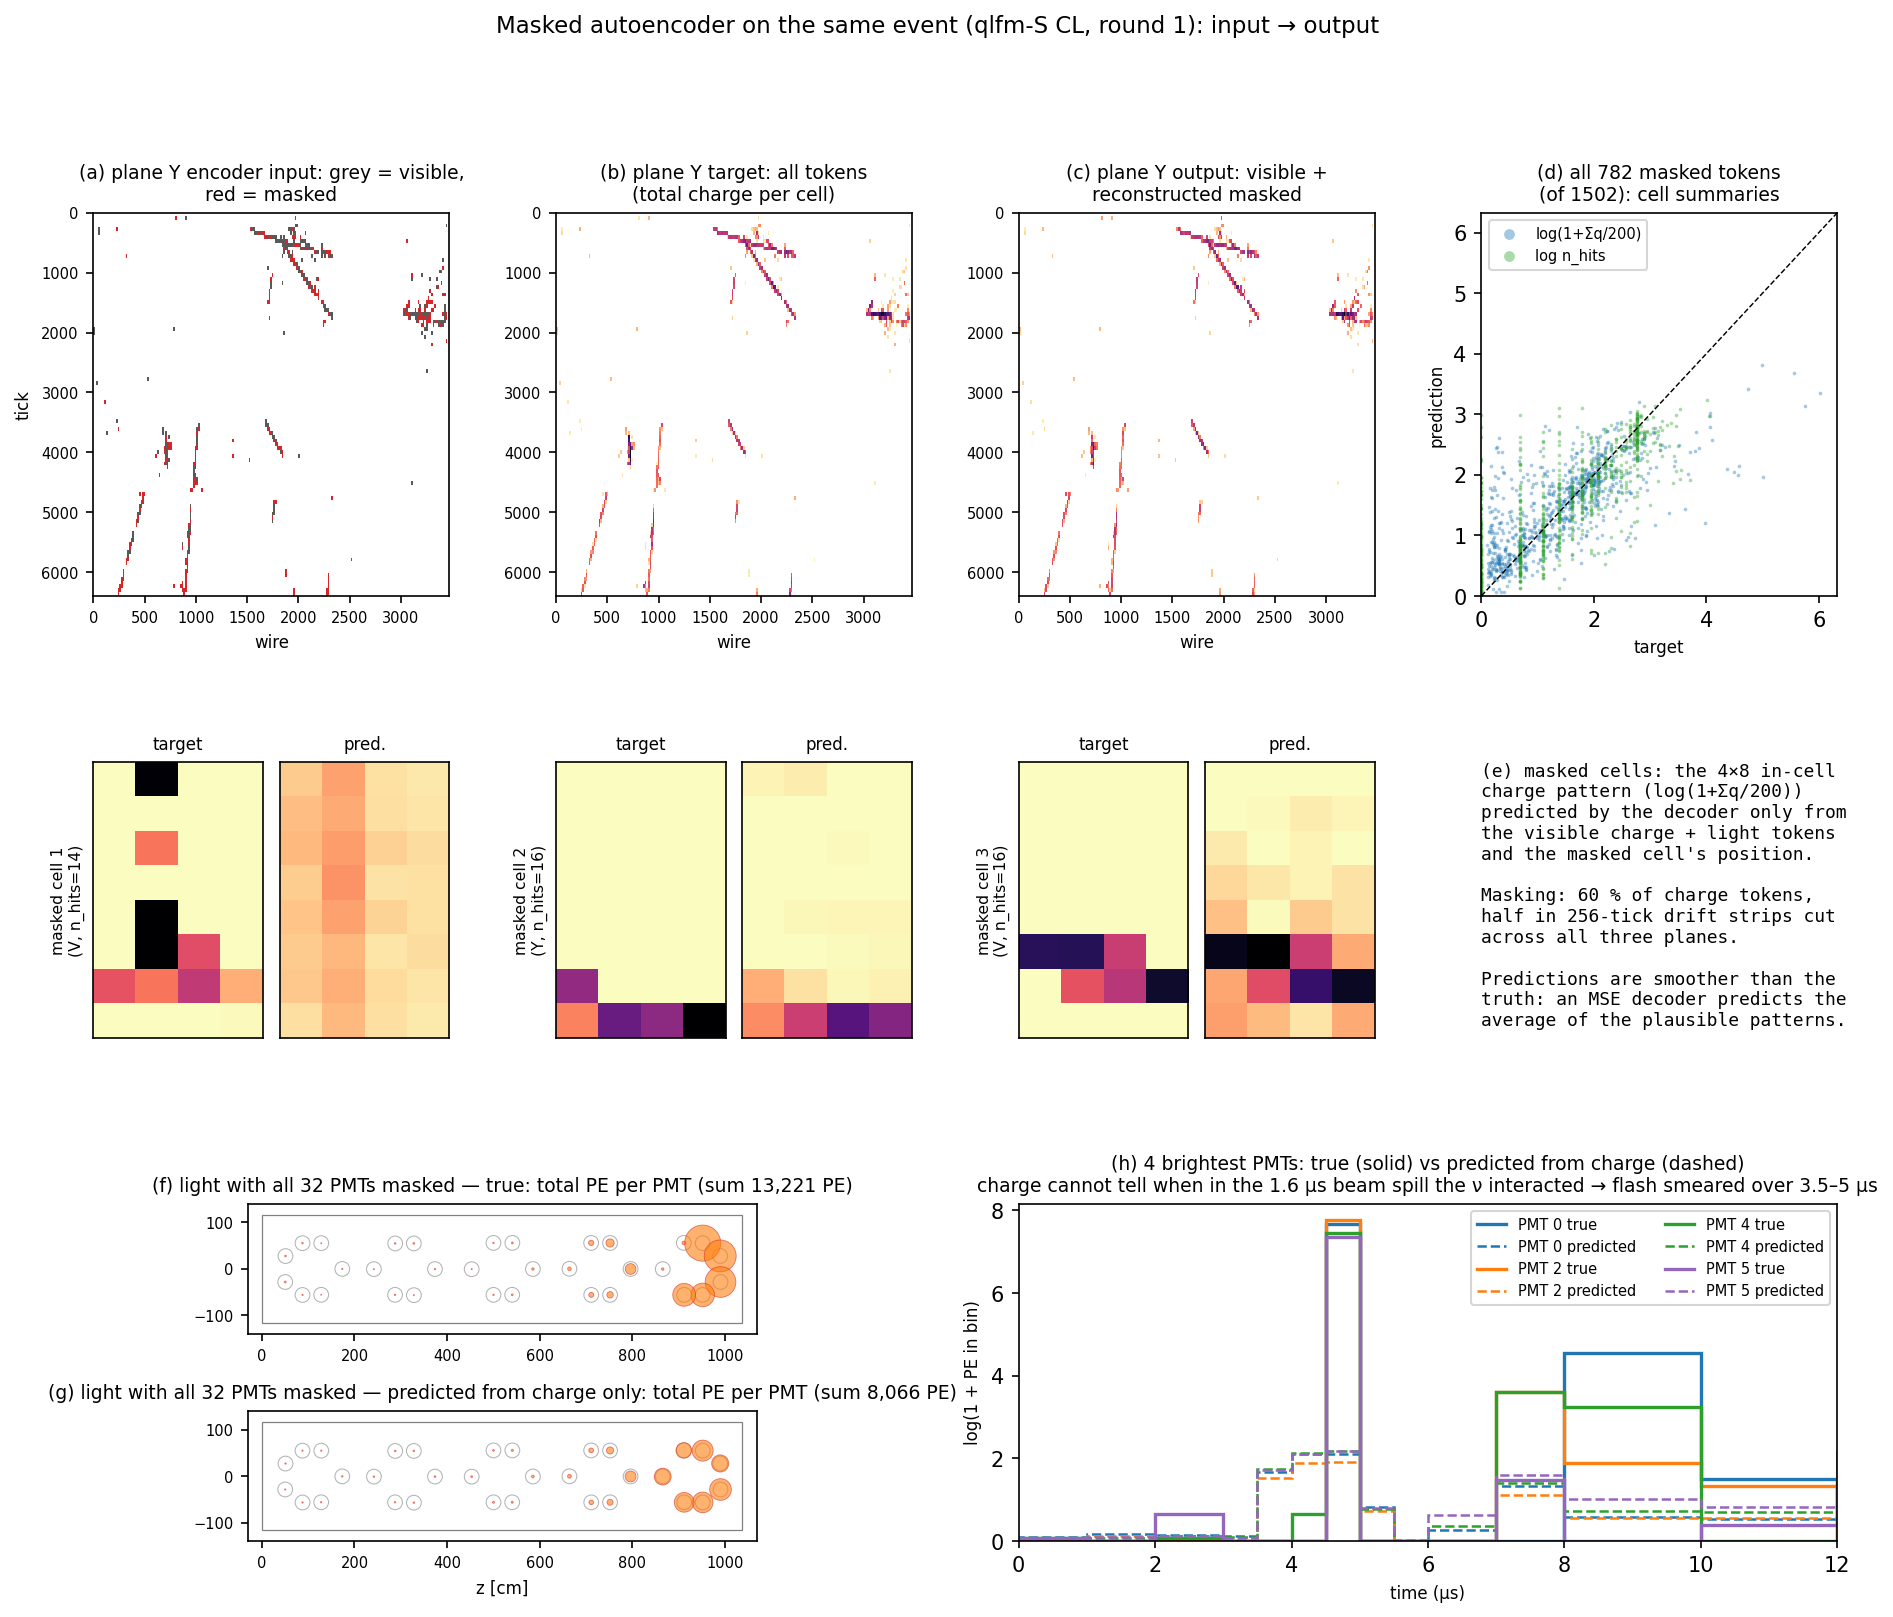
\includegraphics[width=0.85\textwidth]{../figures/r1_mae_io.png}
\caption{\demo{} (TN1 Fig.~5). Masked-autoencoder input and output for one event. {\color{plan}Final: model overview -- charge cells and PMT tokens $\to$ shared Transformer $\to$ MAE decoder / task heads.}}\label{fig:model}
\end{figure}

%=====================================================================
\section{Light helps, and learning the correlation is key}\label{sec:light}
\subsection{Pretraining works and light helps}
\begin{figure}[H]\centering
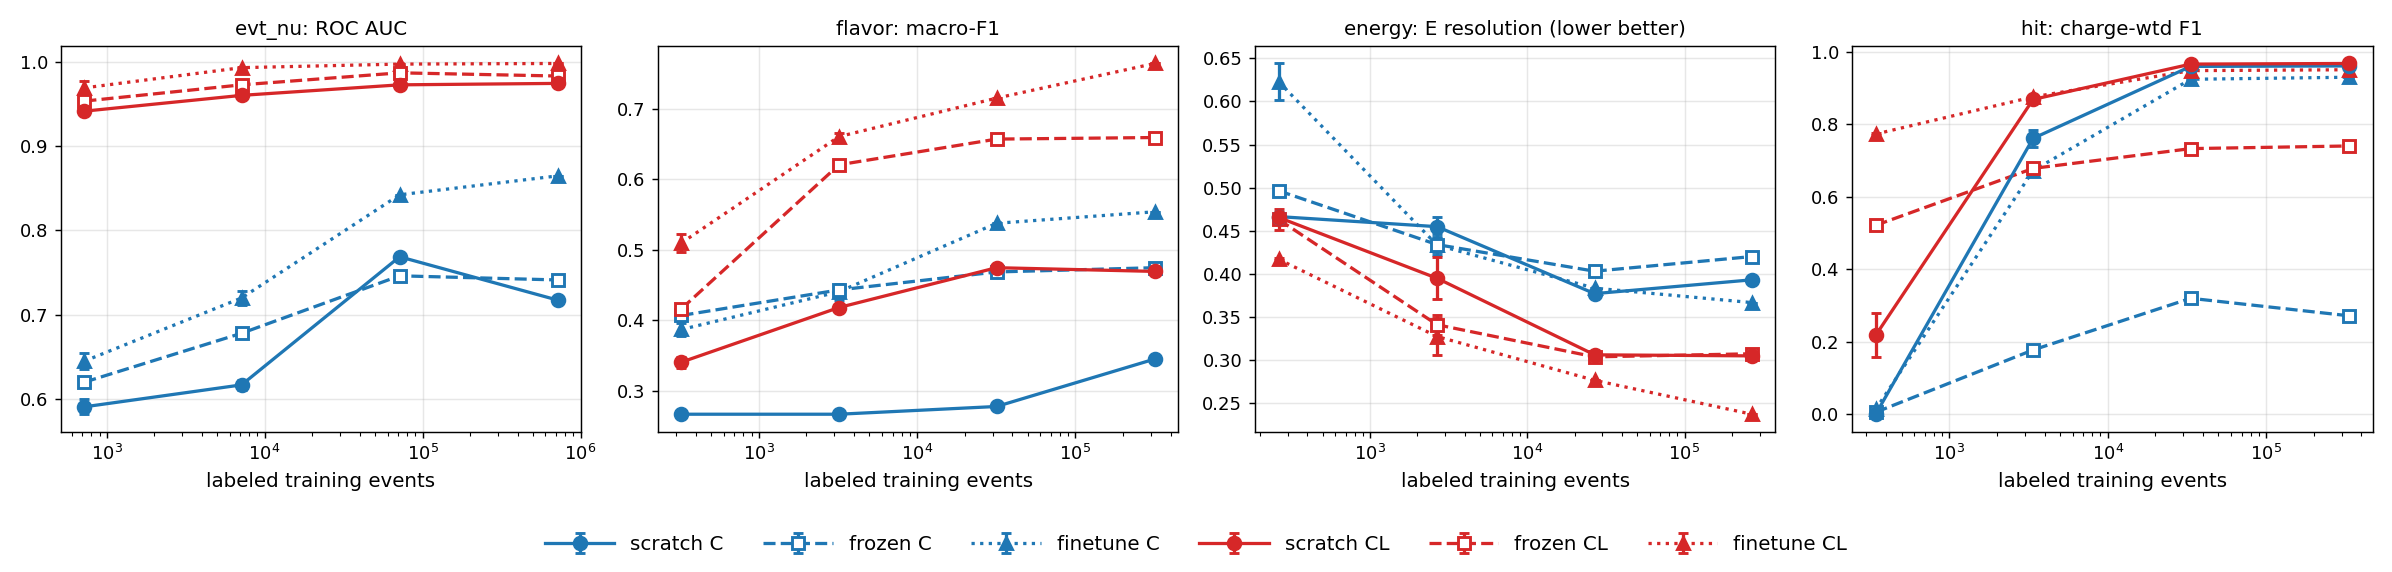
\includegraphics[width=\textwidth]{../figures/e3_label_efficiency.png}
\caption{\demo{} (TN1 Fig.~6, 6.6M models). Test metrics vs labelled events; blue charge only (C), red charge + light (CL); scratch, frozen and fine-tuned. {\color{plan}Final: qlfm-M CL vs qlfm-M C only (21M), the updated metrics of Table~\ref{tab:tasks}, five panels (T1--T5), frozen and multi-task fine-tune.}}\label{fig:light}
\end{figure}

\subsection{Correlations from pretraining beat light added afterwards}
\begin{figure}[H]\centering
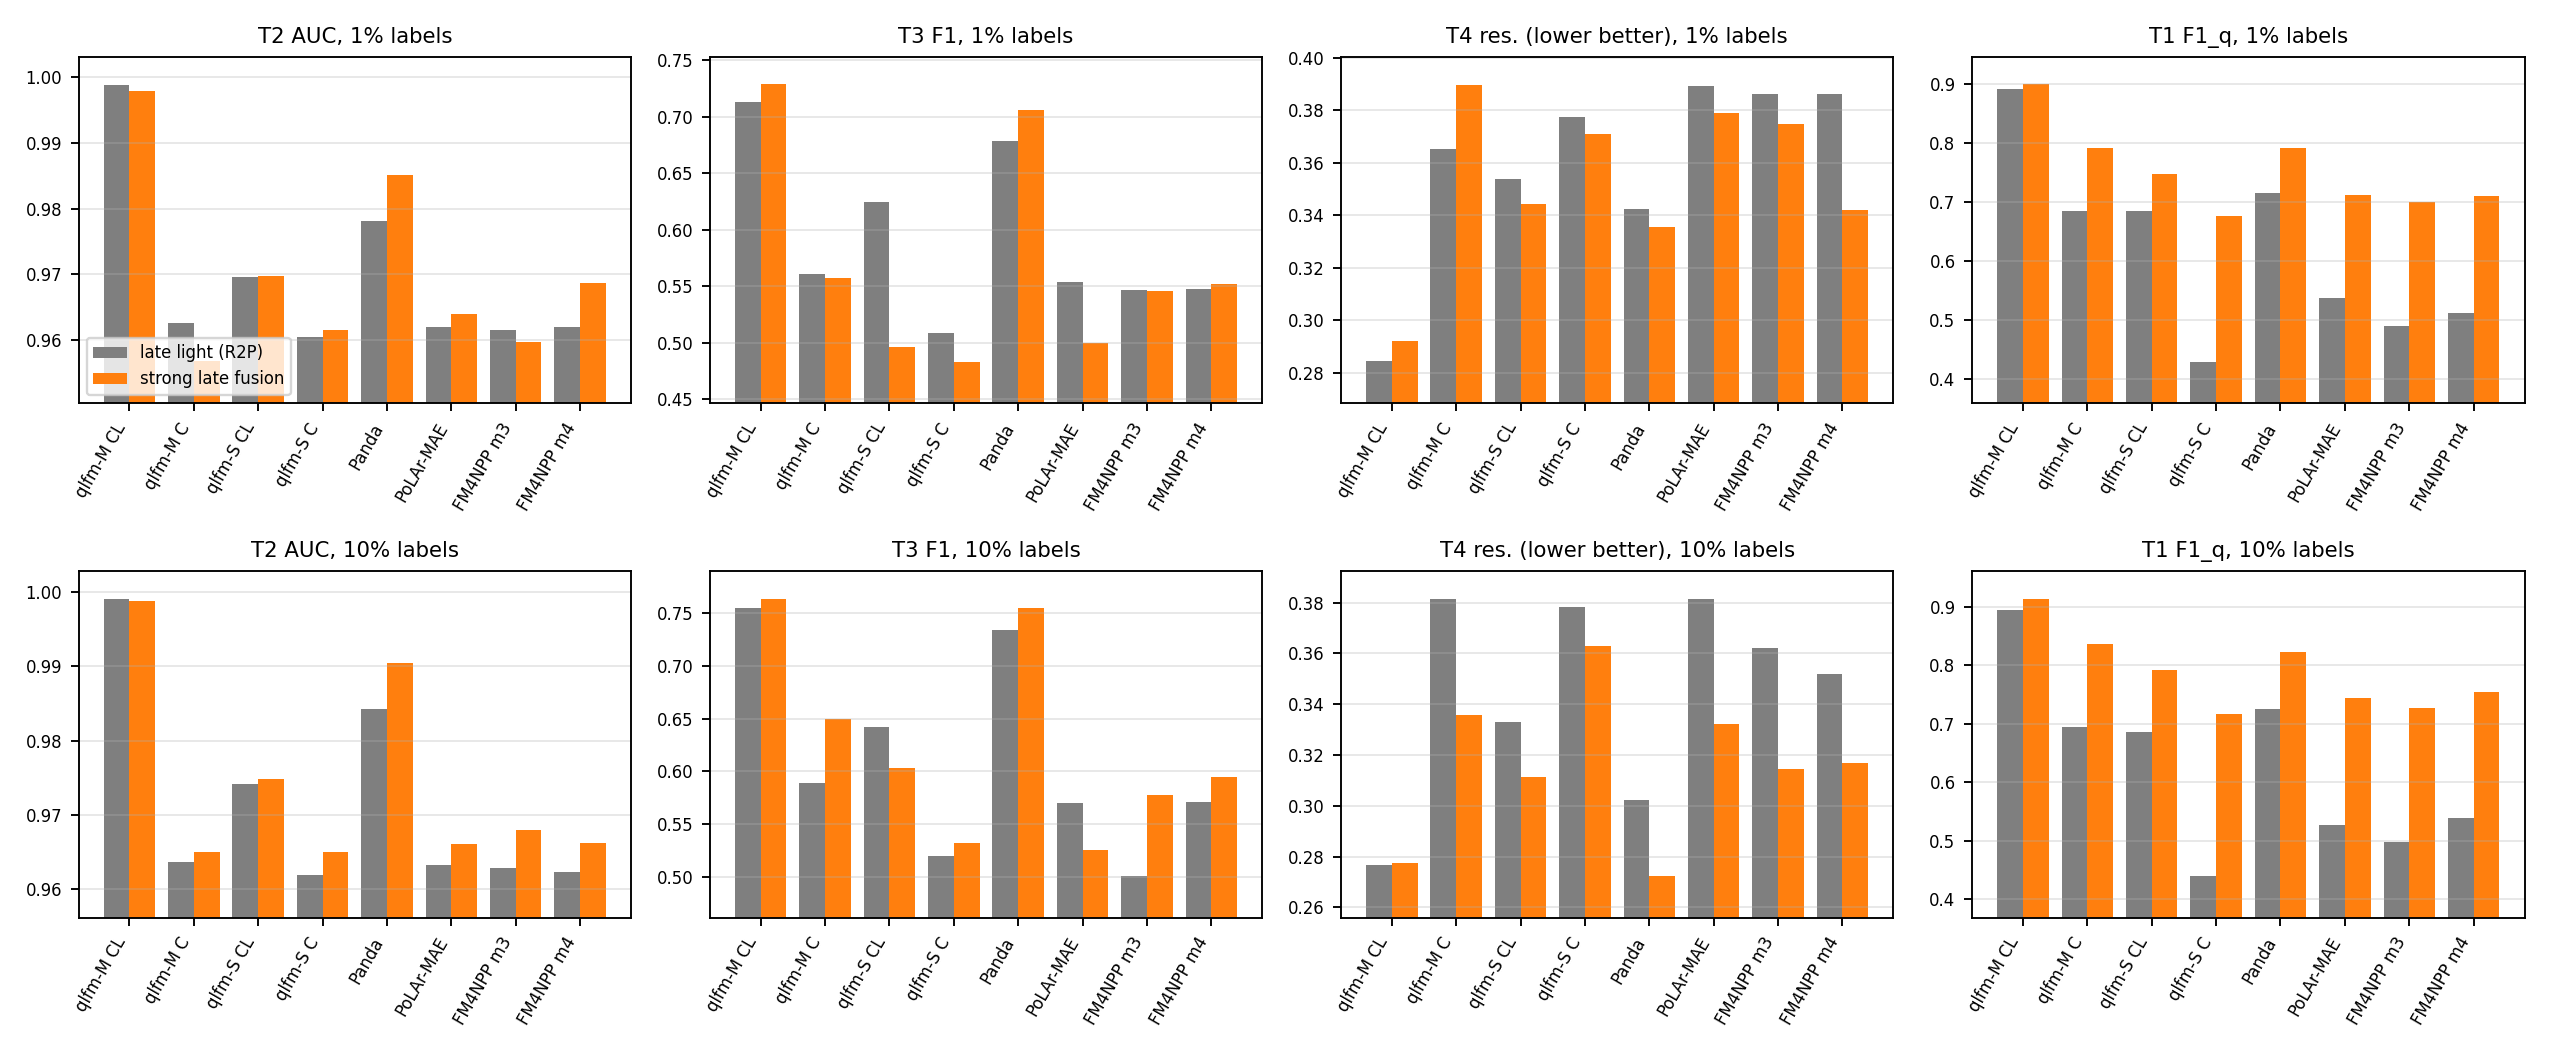
\includegraphics[width=\textwidth]{../figures/round3_fusion.png}
\caption{\demo{} (TN3). Frozen backbones at 1\% (top) and 10\% labels (bottom) with weak late light (grey) and strong late fusion (orange, cross-attention from charge to PMT tokens). qlfm-M CL has light in pretraining; all other backbones are charge-only. {\color{plan}Final: keep, restrict to qlfm-M CL, qlfm-M C, PTv3 + Sonata; updated metrics.}}\label{fig:fusion}
\end{figure}

\begin{table}[H]\centering\small
\caption{\demo{} values from TN2--4 (frozen, 1\% labels, seed 0; T1 charge-weighted median per-event F1; T2 on the 200\,PE pass sample; T4 on all CC fiducial events). Late fusion = strong cross-attention head. {\color{plan}Final: 0.1\% and 1\% labels, frozen and multi-task fine-tune, updated metrics, 3 seeds; C-only diagnostic rows (light removed at inference).}}\label{tab:main}
\begin{tabular}{llccccc}\toprule
Model & Light & T1 F1 $\uparrow$ & T2 AUC $\uparrow$ & T3 F1 $\uparrow$ & T4 res.\ $\downarrow$ & T5 MSE $\downarrow$\\\midrule
qlfm-M CL & pretraining & \textbf{0.91} & \textbf{0.99} & \textbf{0.713} & \textbf{0.284} & \textbf{0.503}\\
qlfm-M C & late head & 0.80 & 0.82--0.86 & 0.558 & 0.390 & 0.586\\
PTv3 + Sonata & late head & 0.79 & 0.95--0.97 & 0.706 & 0.336 & 0.577\\
Pandora (+ BDT) & BDT features & 0.81 & 0.95 & 0.559 & 0.400 & n/a\\
\bottomrule\end{tabular}
\end{table}

\subsection{Shortcut control and charge$\to$light prediction}
The large-light cut (T2) and the charge-only T5 task test whether the model uses charge--light consistency rather than the presence of a flash. qlfm-M CL predicts the PMT light from charge alone, and its own MAE decoder does so with no labels at all (MSE 0.506 vs 0.503 with a trained head; charge-only encoders 0.58--0.59).
\begin{figure}[H]\centering
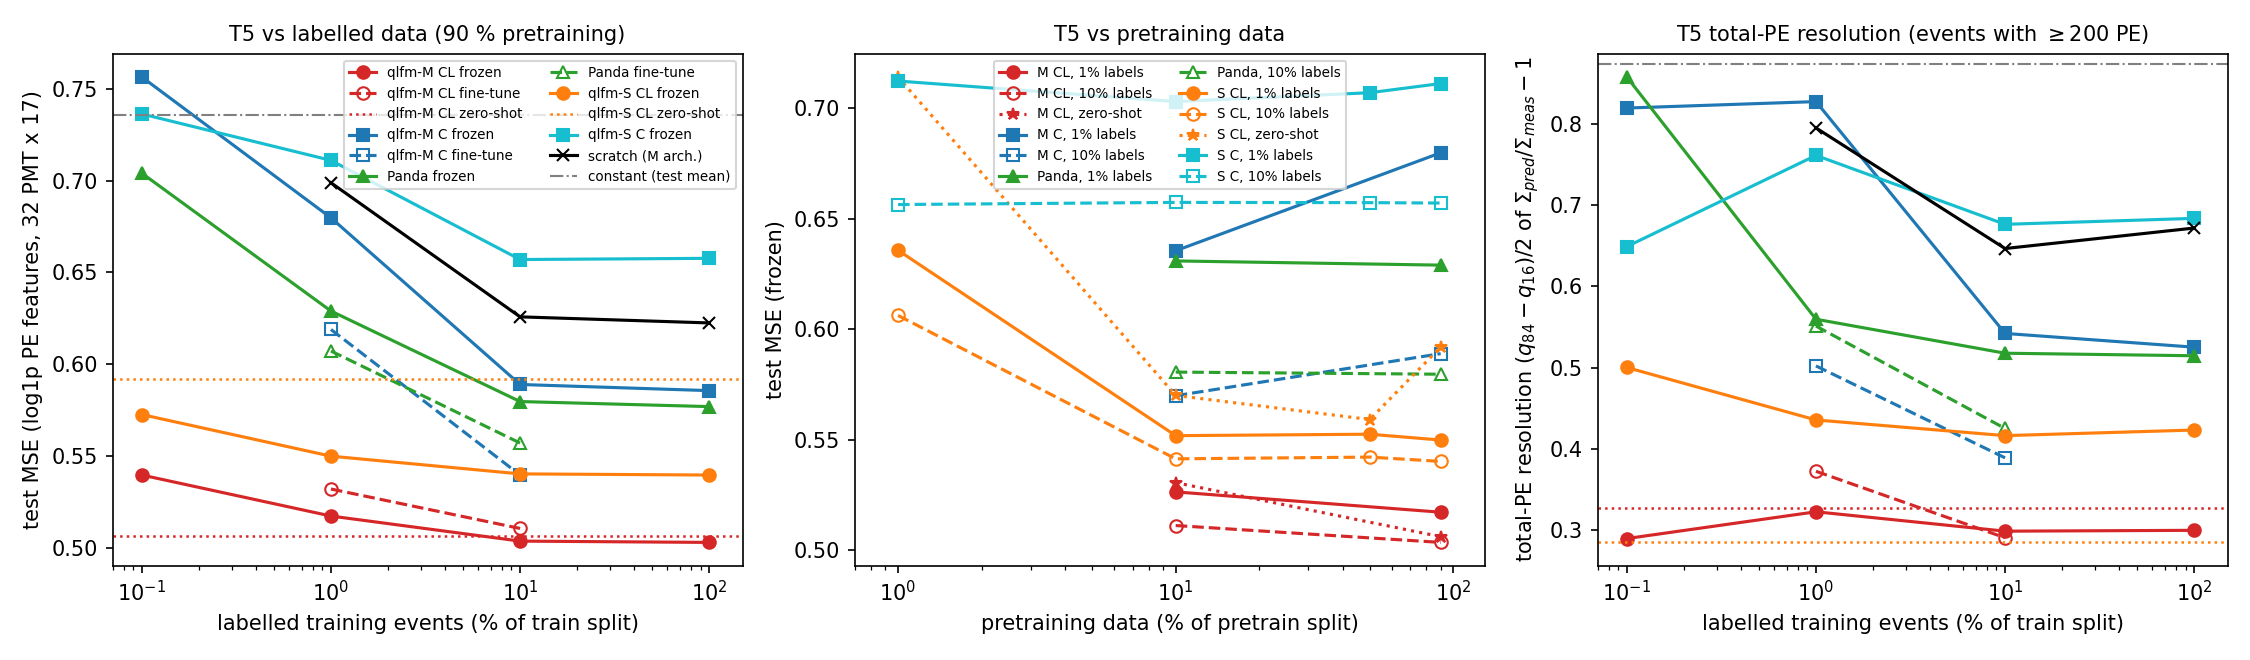
\includegraphics[width=0.49\textwidth]{../figures/round4_t5_scaling.png}\hfill
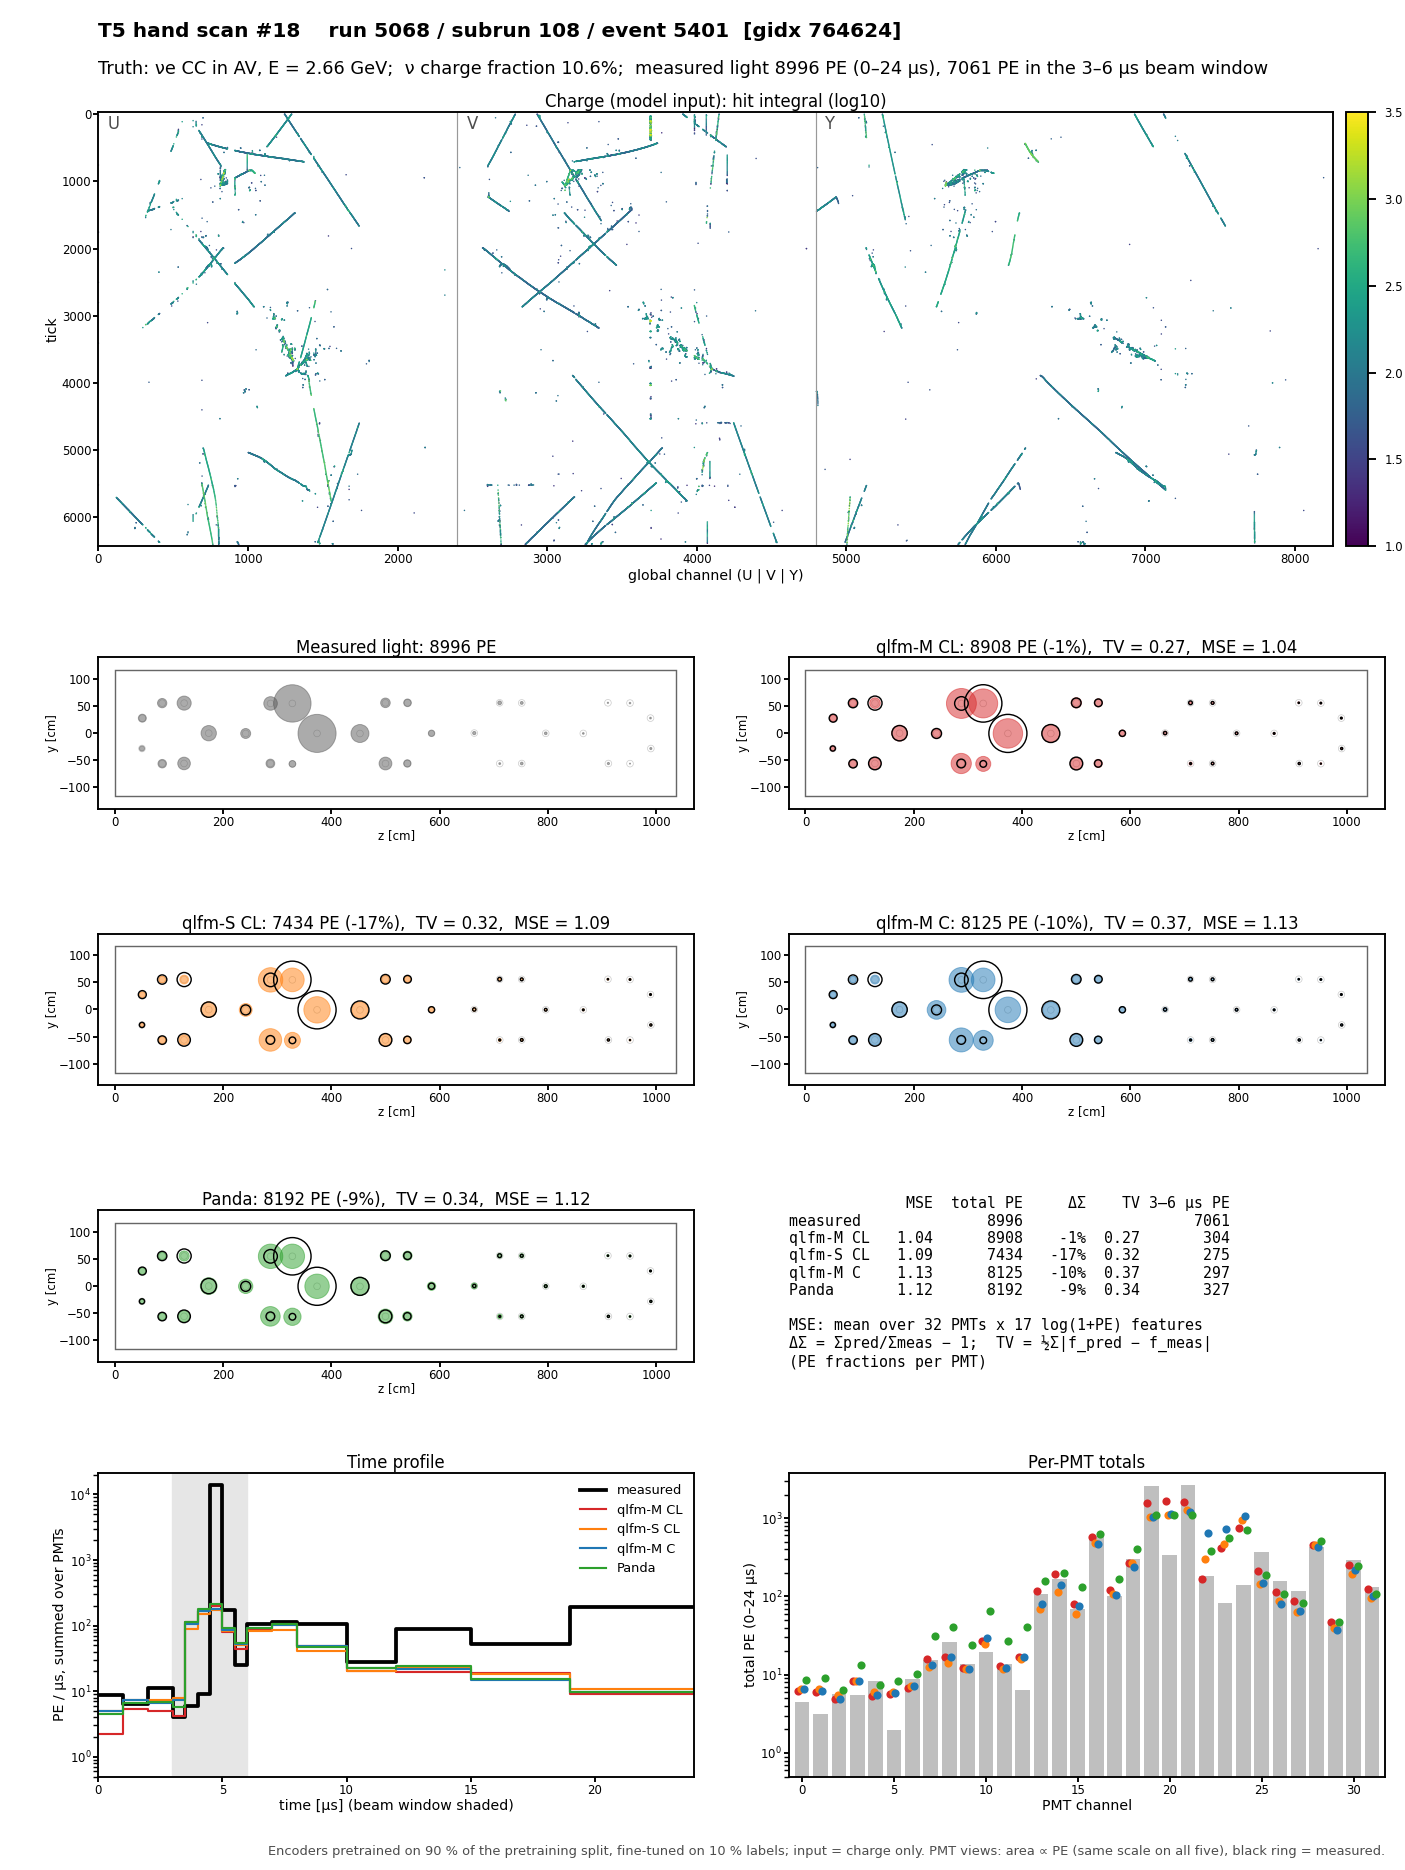
\includegraphics[width=0.49\textwidth]{fig/demo_t5_hs18.png}
\caption{\demo{} (TN4). Left: T5 test MSE vs pretraining and label fraction. Right: one hand-scan event (measured vs predicted PMT light). {\color{plan}Final: T5 bar chart for the four models + zero-shot, and one display.}}\label{fig:t5}
\end{figure}

\subsection{Multi-task fine-tuning}
\todo{New. One backbone, five heads; loss per task masked to its eligible events, weights normalized by each task's initial loss. Compare with single-task fine-tunes at 0.1\% and 1\%: how much does sharing the backbone cost?}
\begin{table}[H]\centering\small
\caption{\demo{} layout. Single-task (ST) vs multi-task (MT) fine-tune, qlfm-M CL. {\color{plan}Values pending.}}\label{tab:mt}
\begin{tabular}{llccccc}\toprule
Labels & Fine-tune & T1 & T2 & T3 & T4 & T5\\\midrule
0.1\% & ST / MT & -- / -- & -- / -- & -- / -- & -- / -- & -- / --\\
1\% & ST / MT & -- / -- & -- / -- & -- / -- & -- / -- & -- / --\\
\bottomrule\end{tabular}
\end{table}

%=====================================================================
\section{Which multi-modal FM architecture suits LArTPCs?}\label{sec:arch}
So far only qlfm saw light in pretraining; the references got light only at the head. Other recipes may absorb the charge--light correlation better. We give each recipe light in pretraining and compare at matched size ($\approx$20M) and compute (20 node-hours of pretraining).

\begin{table}[H]\centering\footnotesize
\caption{The four recipes. Architecture and objective change together except for the MAE/JEPA pair, which isolates the objective on one backbone.}\label{tab:recipes}
\begin{tabularx}{\textwidth}{lllL}\toprule
Recipe & Backbone & Objective & How light enters pretraining\\\midrule
qlfm-M CL & Transformer & MAE (charge + light) & PMT tokens in the sequence (as now)\\
qlfm-M CL JEPA & Transformer & JEPA (I-JEPA-style) & same tokens; predictor regresses EMA-target embeddings of masked charge blocks and masked PMTs\\
PTv3 + Sonata + L & PTv3 & self-distillation & event-level cloud: 3 planes plus 32 PMT points in a fourth slab, placed at their $(z,y)$; per-modality input embedding \todo{verify in smoke test}\\
Mamba-2 + L & Mamba-2 (FM4NPP m4) & k-NNN + masked light & PMT tokens as prefix (conditioning) and suffix (masked light regressed from the charge); hits as in FM4NPP\\
\bottomrule\end{tabularx}
\end{table}

\begin{figure}[H]\centering
\ph{4.5cm}{Convergence: validation loss vs epoch for each recipe (own objective), and a frozen probe (T2 bright AUC, T5 MSE) at 2, 5, 10, 20 node-hours -- the only curve comparable across objectives.}
\caption{\demo{} Pending (Appendix~\ref{app:plan}).}\label{fig:conv}
\end{figure}
\begin{table}[H]\centering\small
\caption{\demo{} layout. Multi-task fine-tune at 1\% labels (selection metric), and frozen at 1\%; 3 seeds.}\label{tab:arch}
\begin{tabular}{lcccccc}\toprule
Recipe & T1 & T2 & T3 & T4 & T5 & mean rank\\\midrule
qlfm-M CL (MAE) & -- & -- & -- & -- & -- & --\\
qlfm-M CL (JEPA) & -- & -- & -- & -- & -- & --\\
PTv3 + Sonata + L & -- & -- & -- & -- & -- & --\\
Mamba-2 + L & -- & -- & -- & -- & -- & --\\
\bottomrule\end{tabular}
\end{table}

%=====================================================================
\section{How the correlations are learned}\label{sec:how}
\begin{itemize}
  \item \textbf{Embedding maps.} t-SNE / PCA of frozen event and token embeddings without a learned map, coloured by $\nu$/cosmic, flavour, energy, drift coordinate (as FM4NPP Fig.~8~\cite{fm4npp}).
  \item \textbf{Probes.} Linear probes on charge tokens only (light masked at inference) for the drift coordinate $x$ (which needs $t_0$), deposited energy and the vertex: CL vs C encoder.
  \item \textbf{Fusion depth} (survey E1). Light enters at the input, after $L/2$ blocks, or only at the head, all at matched compute.
  \item \textbf{Oracle 3D input} {\color{plan}(appendix-level).} The open data has no space points; a 3D input can only be truth energy deposits. It gives an upper bound on what 3D reconstruction could add, and is labelled as an oracle.
  \item \textbf{Light-swap counterfactual} (survey E2, optional): replace an event's light by another event's and measure the drop.
  \item \textbf{Validity checks} (Josh Peterson's survey round 1.5, after Aobo Li's papers; inference only, $<$1\,nh each):
  shuffled-label and plane/PMT-group ablations on T1/T2 (A2); MAE reconstruction loss vs T2 score for $\nu$ and cosmic events, to rule out an internal shortcut (A5); T1 efficiency vs drift coordinate, wire plane and hit amplitude (A3); data vs simulation: T5 errors on no-$\nu$ events (real off-beam cosmic light) vs $\nu$ events (simulated light) (A1, partial: no beam-off sample in the open data).
\end{itemize}
\begin{figure}[H]\centering
\ph{3.5cm}{t-SNE of frozen event embeddings, qlfm-M CL vs qlfm-M C (pending).}
\caption{\demo{} Pending.}\label{fig:tsne}
\end{figure}

%=====================================================================
\section{Scaling} \label{sec:scaling}
{\color{plan}On hold until Sections 3--5 are done and the go-ahead is given.} Scaling of each recipe with model size and compute; smaller charge cells (more tokens), where SSMs may gain (Josh's SSM survey).

\section{Discussion and limitations}
Overlay simulation (no beam-on data); one detector; models of about 20M parameters; compute-limited training; T4 on a clean subset. \todo{expand.}

%=====================================================================
\appendix
\section{Model setups}\label{app:models}
\todo{One subsection per recipe: tokenizer, backbone, objective, hyper-parameters, pretraining compute, heads; MAE input/output and token figures from TN1 (Figs.~2--4).}

\section{Event displays}\label{app:displays}
\begin{figure}[H]\centering
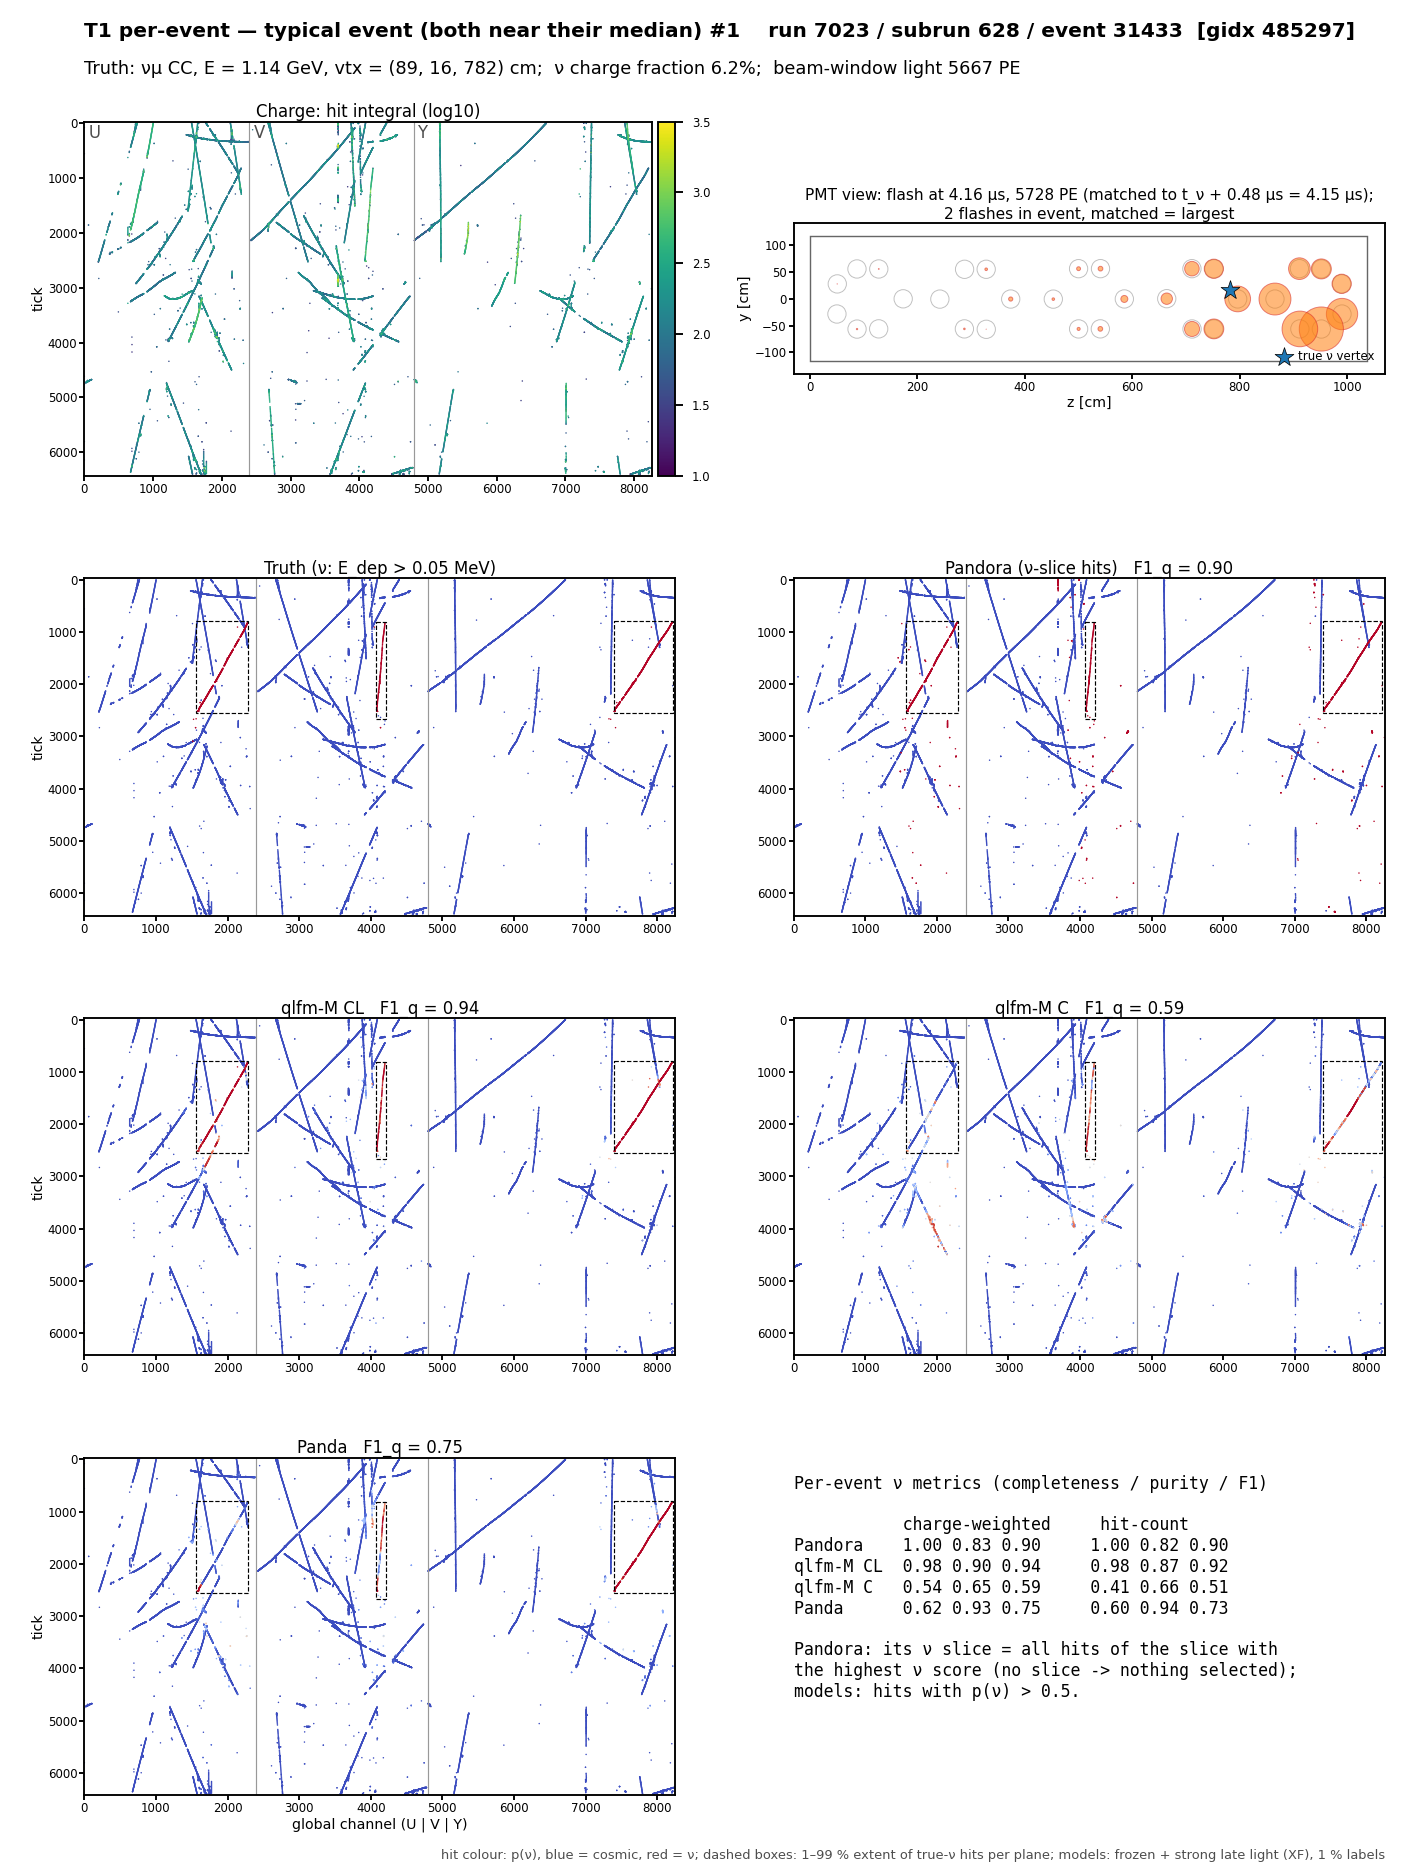
\includegraphics[width=\textwidth]{fig/demo_t1_typical01.png}
\caption{\demo{} (TN4). A typical event: T1 hit predictions of qlfm-M CL, qlfm-M C, PTv3 and Pandora.}\label{fig:disp}
\end{figure}

%=====================================================================
\section{Campaign plan}\label{app:plan}
\subsection{Decisions so far (6 Nov 2026)}
\begin{itemize}
  \item Section~\ref{sec:arch} first; total budget $\leq$200 node-hours (nh), charged to \code{neutrinoGPU::WireCellDev}, preemptable queue.
  \item All four recipes pretrained at the same budget, 20\,nh each, including a new qlfm-M CL run (the existing one used about 2\,nh, the round-2 references about 4\,nh).
  \item T4 scored on a truth-based subset common to all models (not on each model's T1): $\nu$ share of the event charge $\geq$5\%, visible fraction $\geq$0.3.
  \item Benchmark release (splits, tasks, metrics, baselines). Josh Peterson's code audit is fixed before any campaign run; his checks A1--A5 go into Section~\ref{sec:how}.
  \item JEPA on the qlfm Transformer, so MAE vs JEPA isolates the objective.
  \item ``Reco-3D'' becomes an oracle study with truth deposits (no space points in the open data).
  \item Naming: PTv3 + Sonata (``as used in Panda''), not ``Panda'' and not ``PT2''.
  \item Venue: ICML 2027 main conference, \emph{Application-Driven ML} area (deadline expected late January 2027); fallbacks: an ICML 2027 workshop, the NeurIPS 2027 Datasets \& Benchmarks track, MLST.
\end{itemize}

\subsection{Section~\ref{sec:arch} job plan}
\paragraph{Step 0 -- code (login node + short debug jobs).}
\begin{enumerate}
  \item Multi-task fine-tune mode in \code{train\_downstream} (five heads, masked per-task losses, loss normalization); works for all backbones through the common interface.
  \item Light for PTv3: event-level clouds (3 planes + PMT points), Sonata views include PMTs; pretraining config \code{ptv3\_sonata\_cl}.
  \item Light for Mamba-2: PMT prefix and suffix tokens, masked-light regression added to the k-NNN loss.
  \item JEPA objective on the qlfm backbone (context encoder, EMA target encoder, narrow predictor; block masks on each plane plus masked PMTs); collapse monitor (embedding rank).
  \item Logging: validation loss every $\approx$15 minutes; checkpoints kept at 2, 5, 10, 20\,nh for the probe curve.
\end{enumerate}
qlfm-M CL needs no new code and starts first.

\paragraph{Step 1 -- smoke tests.} 30-minute runs of each new recipe: loss falls, no NaN, throughput measured (sets the step count for 20\,nh), resume after a kill works.

\paragraph{Step 2 -- pretraining.} Four 1-node preemptable jobs of 20\,h each (\code{-r y}, resumable), running in parallel; the feeder keeps at most 6 jobs in the queue.

\paragraph{Step 3 -- downstream.} For each recipe, using the 1-node \code{queue.pbs} worker (4 tasks per node):
\begin{itemize}
  \item frozen heads, T1--T5, at 0.1\% and 1\%;
  \item multi-task fine-tune at 0.1\% and 1\%, 3 seeds (selection metric: 1\%);
  \item single-task fine-tunes of qlfm-M CL at 1\% (for Table~\ref{tab:mt});
  \item probe curve: frozen T2 and T5 at 1\% on the 2/5/10/20\,nh checkpoints.
\end{itemize}

\begin{table}[H]\centering\small
\caption{Budget for Section~\ref{sec:arch} (node-hours). Downstream costs from rounds 1--4: a frozen or single-task head run takes 0.1--0.3\,nh per GPU slot (4 per node); PTv3 fine-tunes are about 2$\times$ slower.}\label{tab:budget}
\begin{tabular}{lrrl}\toprule
Item & per recipe & total & note\\\midrule
Code and smoke tests & 3--4 & 13 & debug queue\\
Pretraining & 20 & 80 & preemptable, 1 node $\times$ 20 h\\
Probe curve (4 ckpts, T2+T5) & 1.5 & 6 & \\
Frozen heads (5 tasks, 2 fractions) & 1.5 & 6 & \\
Multi-task FT (2 fractions, 3 seeds) & 3--5 & 16 & \\
Single-task FT (qlfm-M CL, 1\%) & -- & 2 & for Table~\ref{tab:mt}\\
Reruns, preemption (about 25\%) & -- & 30 & \\\midrule
\textbf{Total} & & \textbf{$\approx$155} & cap 200 (45 spare)\\
\bottomrule\end{tabular}
\end{table}
The 45\,nh spare can pay for charge-only twins of the new recipes or for the fusion-depth ablation of Section~\ref{sec:how}.

\subsection{Timeline (target)}
\begin{tabular}{ll}
Week of 9 Nov & Step 0--1; qlfm-M CL 20\,nh pretraining starts\\
16--29 Nov & PTv3 + L, Mamba-2 + L, JEPA pretraining\\
30 Nov -- 13 Dec & downstream, probe curves; Section~\ref{sec:arch} results\\
14 Dec -- 10 Jan & Section~\ref{sec:light} updates (metrics, multi-task FT), Section~\ref{sec:how}\\
11--27 Jan & writing; ICML deadline (expected late January)\\
\end{tabular}

\subsection{Risks}
\begin{itemize}
  \item \textbf{PTv3 + L design} (PMT points in a point-cloud backbone) and Sonata's view augmentations may not suit PMT points; fall back to a light cross-attention adapter inside the encoder stages (mid fusion) and say so.
  \item \textbf{JEPA collapse}: our earlier self-distillation on qlfm tokens (qlfm-SD) underperformed, probably due to a low learning rate; monitor embedding rank, tune the LR in the smoke test.
  \item \textbf{Mamba-2 and masking}: SSMs fit MAE poorly (Josh's SSM survey); we keep FM4NPP's k-NNN objective and add masked light at the suffix.
  \item \textbf{Preemption}: runs resume from checkpoints; validated only with a normal job so far.
\end{itemize}

%=====================================================================
\begin{thebibliography}{99}\small
\bibitem{mpm} T.~Golling et al., Masked particle modeling on sets, MLST (2024), arXiv:2401.13537.
\bibitem{mpmv2} M.~Leigh et al., Is tokenization needed for masked particle modelling?, MLST (2025), arXiv:2409.12589.
\bibitem{polarmae} S.~Young et al., Particle trajectory representation learning with masked point modeling (PoLAr-MAE), arXiv:2502.02558.
\bibitem{panda} S.~Young, K.~Terao, Panda: self-distillation of reusable sensor-level representations for high energy physics, arXiv:2512.01324.
\bibitem{pandav2} S.~Young, C.~Jes\'us-Valls, K.~Terao, Panda Diplomacy, arXiv:2609.00611.
\bibitem{fm4npp} D.~Park, S.~Li, Y.~Huang et al., FM4NPP: a scaling foundation model for nuclear and particle physics, arXiv:2508.14087.
\bibitem{fasercal} S.~Alonso-Monsalve et al., Nature Mach.\ Intell.\ (2026), arXiv:2604.07037.
\bibitem{hallin} A.~Hallin, Foundation models for high-energy physics, arXiv:2509.21434.
\bibitem{multimae} R.~Bachmann et al., MultiMAE, ECCV 2022, arXiv:2204.01678.
\bibitem{aion} L.~Parker et al., AION-1, NeurIPS 2025, arXiv:2510.17960.
\bibitem{prompting} N.~Kakati et al., Prompting particle physics, arXiv:2609.31862.
\bibitem{heptokens} J.~Krupa et al., Precision tokenization for multi-modal data in HEP, arXiv:2610.13876.
\bibitem{shukor} M.~Shukor et al., Scaling laws for native multimodal models, ICCV 2025, arXiv:2504.07951.
\bibitem{pandora} R.~Acciarri et al.\ (MicroBooNE), The Pandora multi-algorithm approach to automated pattern recognition of cosmic-ray muon and neutrino events in the MicroBooNE detector, EPJC 78 (2018) 82, arXiv:1708.03135.
\bibitem{mae} K.~He et al., Masked autoencoders are scalable vision learners, CVPR 2022, arXiv:2111.06377.
\bibitem{ijepa} M.~Assran et al., Self-supervised learning from images with a joint-embedding predictive architecture, CVPR 2023, arXiv:2301.08243.
\bibitem{ptv3} X.~Wu et al., Point Transformer V3, CVPR 2024, arXiv:2312.10035.
\bibitem{sonata} X.~Wu et al., Sonata: self-supervised learning of reliable point representations, CVPR 2025, arXiv:2503.16429.
\bibitem{mamba2} T.~Dao, A.~Gu, Transformers are SSMs (Mamba-2), ICML 2024, arXiv:2405.21060.
\end{thebibliography}
\end{document}
